\documentclass[11pt]{article}

\usepackage[margin=1in]{geometry}
\usepackage{graphicx}
\usepackage{booktabs}
\usepackage{amsmath}
\usepackage{hyperref}
\usepackage{float}

\title{Threshold Sensitivity Analysis for Privacy-Preserving Text Routing}
\author{Generated by \texttt{analysis.py}}
\date{}

\begin{document}

\maketitle

\section{Purpose}

This analysis studies how configurable routing thresholds affect the behavior of a
privacy-preserving text routing pipeline. The goal is to understand the tradeoff
between privacy protection and over-flagging. In particular, the analysis focuses
on the problem where non-sensitive samples, such as Wikipedia articles, may be
incorrectly routed as sensitive.

The benchmark labels each sample with an expected binary outcome:
\[
    y = 1
\]
for samples expected to be privacy-critical, and
\[
    y = 0
\]
for samples expected to be non-critical.

A simulated operating point predicts a sample as sensitive if the sample is sent
to either local review or block. A sample is predicted non-sensitive only when it
passes.

\section{Routing Model}

Each sample has a saved joint risk score, a lower-bound $k$-anonymity estimate,
a direct identifier count, and a quasi-identifier count. This script does not
rerun the detector or router. Instead, it simulates alternate decision thresholds
using the saved benchmark fields.

The adjusted risk score is defined as:
\[
    r'(x)
    =
    \mathrm{clip}_{[0,1]}
    \left(
        r(x)
        + w_{direct} \cdot \frac{d(x)}{\max_x d(x)}
        + w_{quasi} \cdot \frac{q(x)}{\max_x q(x)}
    \right),
\]
where $r(x)$ is the saved joint risk score, $d(x)$ is the direct identifier
count, and $q(x)$ is the quasi-identifier count.

The simulated routing rule is:
\[
\mathrm{route}(x) =
\begin{cases}
\mathrm{block}, & k_{lower}(x) < k_{min}, \\\\
\mathrm{block}, & r'(x) \geq \tau_{block}, \\\\
\mathrm{review}, & r'(x) \geq \tau_{review}, \\\\
\mathrm{pass}, & r'(x) < \tau_{review}.
\end{cases}
\]

Thus $\tau_{review}$ controls when a sample first becomes sensitive enough for
local review, while $\tau_{block}$ controls when it is treated as too sensitive
for release. The $k_{min}$ parameter acts as a hard privacy floor.

\section{Dataset Summary}

The analyzed benchmark contains:

\begin{itemize}
    \item Total samples: 600
    \item Expected critical samples: 300
    \item Expected non-critical samples: 300
    \item Positive class rate: 0.500
    \item Wikipedia samples: 300
    \item Wikipedia expected critical samples: 0
    \item Mean joint risk score: 0.125
    \item Mean direct identifier count: 12.392
    \item Mean quasi-identifier count: 4.287
\end{itemize}

\section{Metrics}

The primary privacy metric is recall:
\[
    \mathrm{Recall}
    =
    \frac{TP}{TP + FN}.
\]
In this setting, recall measures the fraction of truly critical samples that
were routed to review or block. Higher recall means stronger privacy protection.

Precision is:
\[
    \mathrm{Precision}
    =
    \frac{TP}{TP + FP}.
\]
Precision measures how often a sensitive routing decision is justified by the
benchmark label.

The false positive rate is:
\[
    \mathrm{FPR}
    =
    \frac{FP}{FP + TN}.
\]
This is especially important for the Wikipedia over-flagging issue, because it
measures how often non-critical samples are incorrectly marked sensitive.

The marked-sensitive rate is:
\[
    \frac{TP + FP}{N}.
\]
This is an operational burden metric. A high marked-sensitive rate means many
samples are being routed to local review or block.

\section{Baseline Operating Point}

The baseline operating point uses:
\[
    \tau_{review}=0.30,
    \quad
    \tau_{block}=0.70,
    \quad
    k_{min}=5,
    \quad
    w_{direct}=0.50,
    \quad
    w_{quasi}=0.50.
\]

The baseline results are:

\begin{center}
\begin{tabular}{lr}
\toprule
Metric & Value \\
\midrule
Precision & 0.869 \\
Recall / privacy protection & 0.663 \\
F1 & 0.752 \\
False positive rate & 0.100 \\
Marked-sensitive rate & 0.382 \\
Pass rate & 0.618 \\
Review rate & 0.210 \\
Block rate & 0.172 \\
\bottomrule
\end{tabular}
\end{center}

\section{Figures}

\subsection{Threshold Phase Diagram}

Figure~\ref{fig:phase} shows how $\tau_{review}$ and $\tau_{block}$
jointly affect recall, false positive rate, review rate, and block rate. This
figure is intended to reveal threshold regions where privacy recall remains high
while false positives decrease.

\begin{figure}[H]
\centering
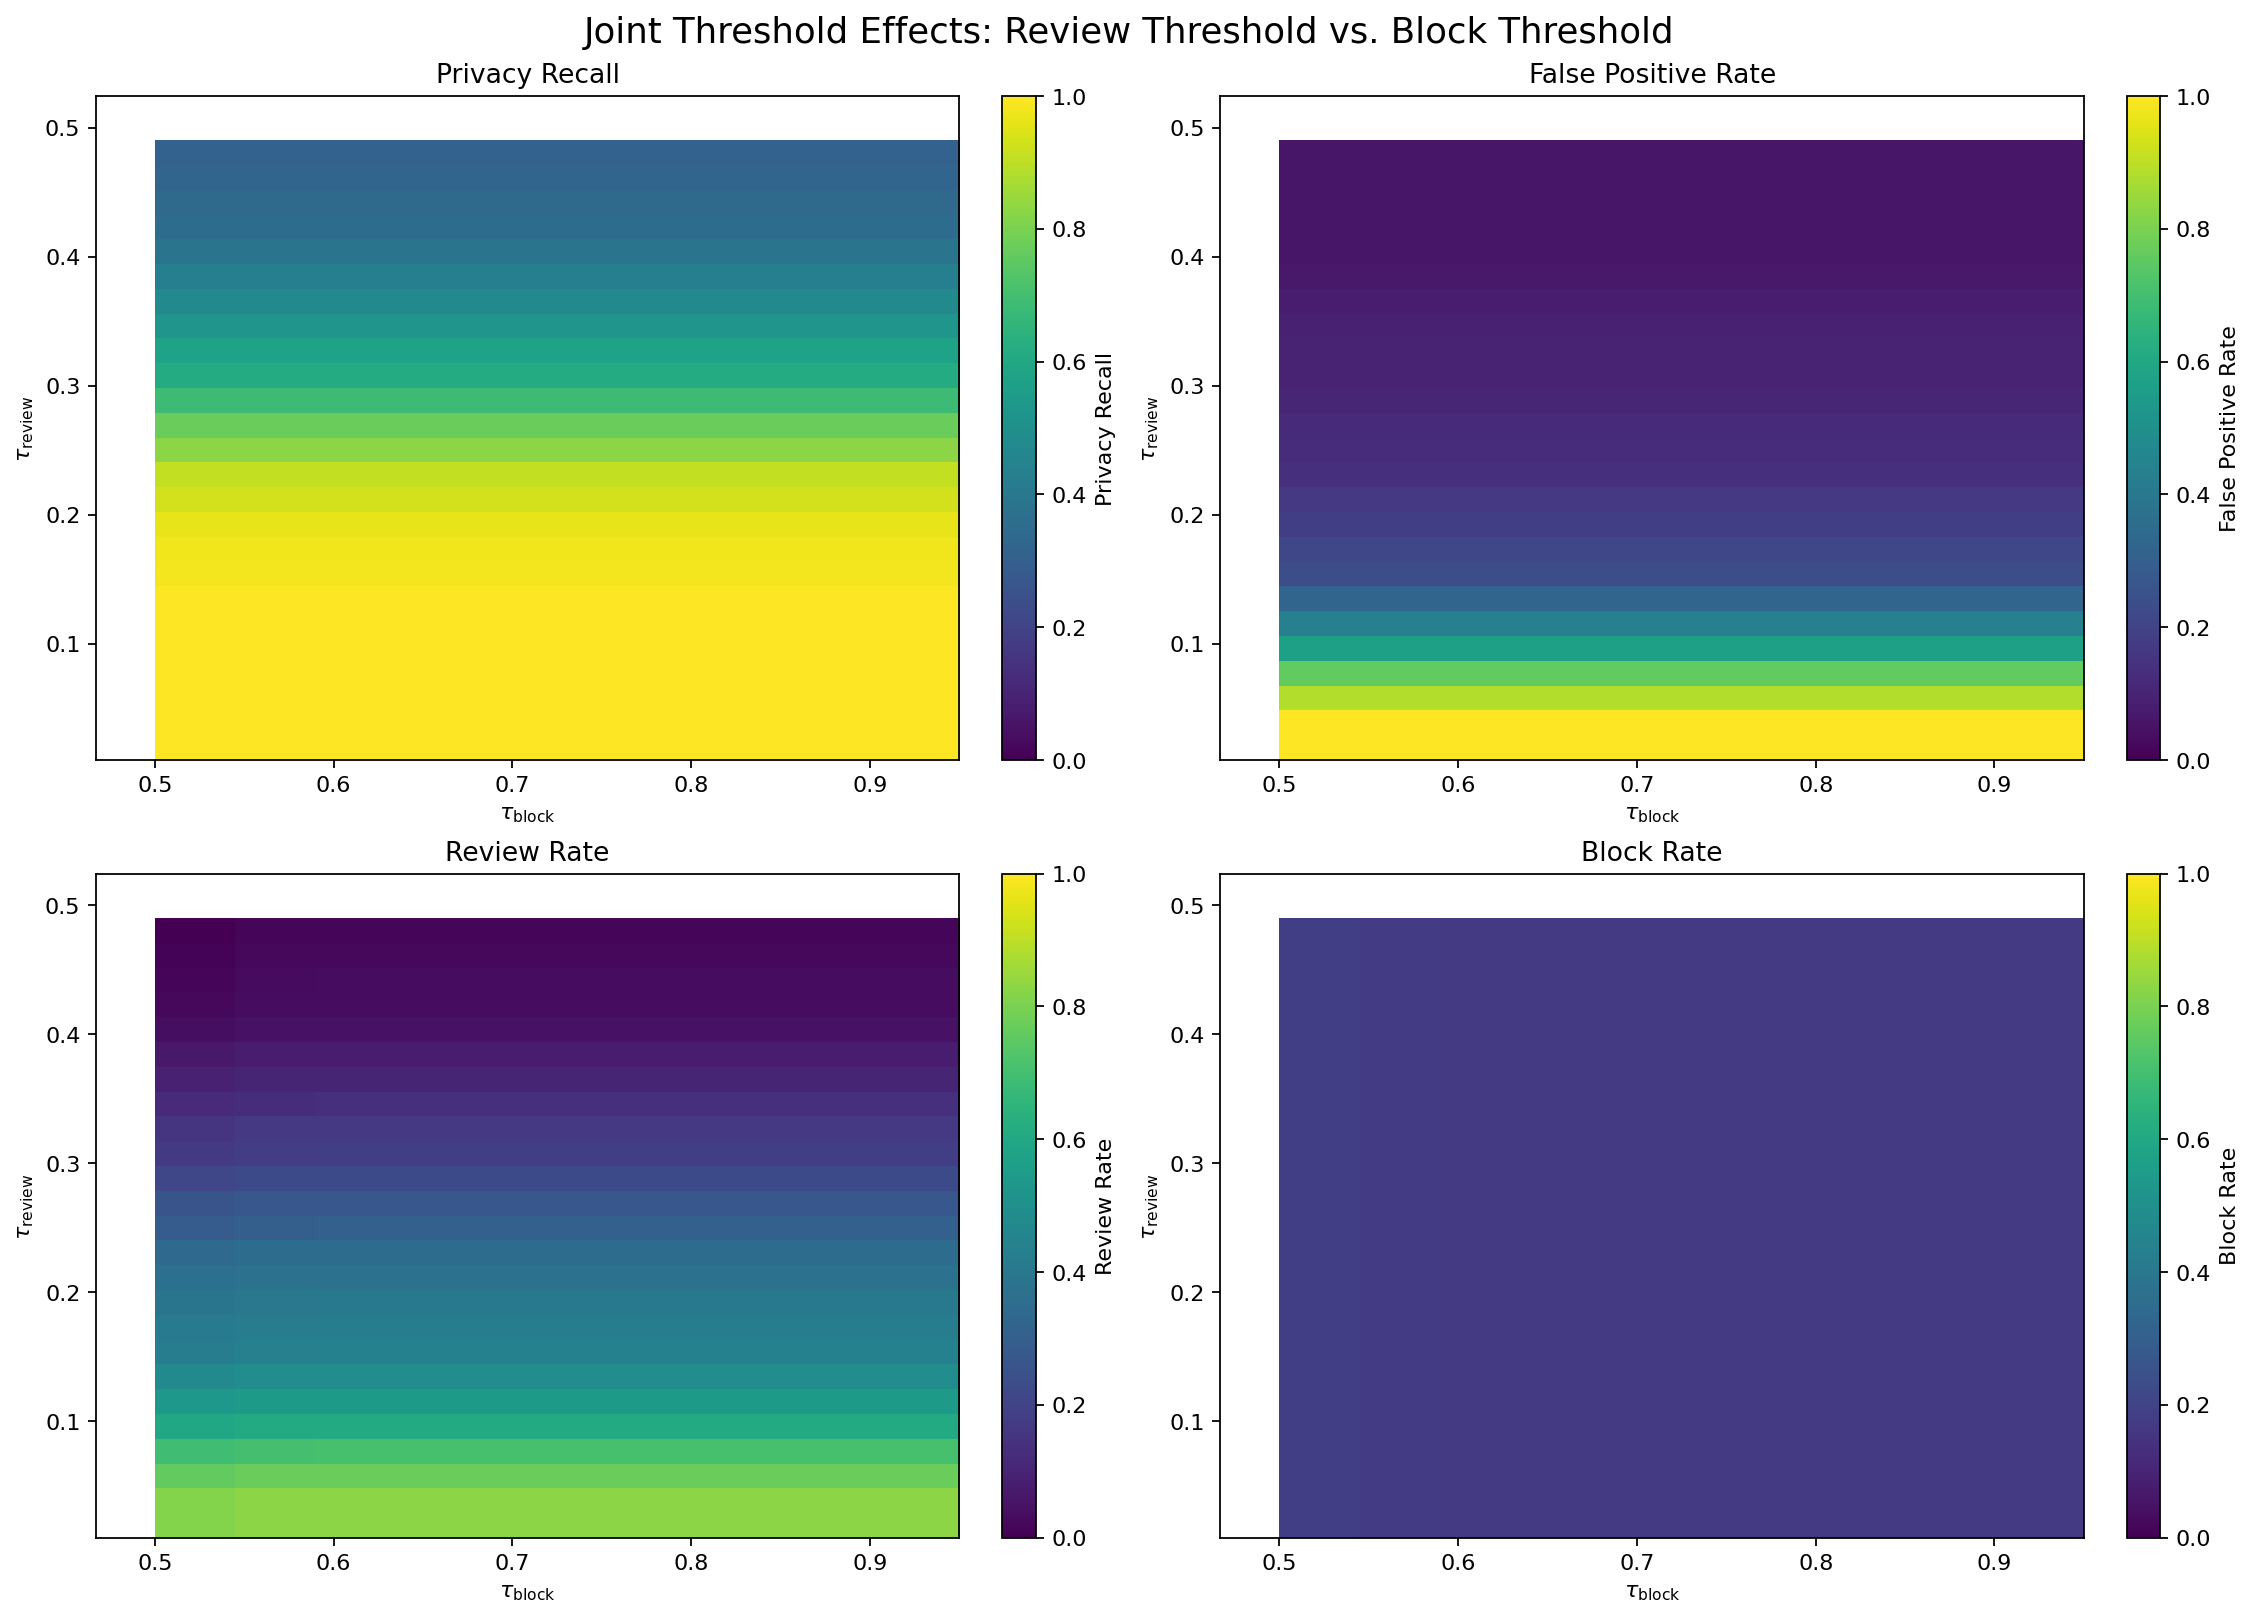
\includegraphics[width=\textwidth]{01_threshold_phase_diagram.png}
\caption{Joint effects of review and block thresholds.}
\label{fig:phase}
\end{figure}

\subsection{Precision-Recall Curves}

Figure~\ref{fig:pr} shows precision-recall behavior across multiple parameter
families. Points are colored by false positive rate, so the desirable region is
high recall, high precision, and low false positive rate.

\begin{figure}[H]
\centering
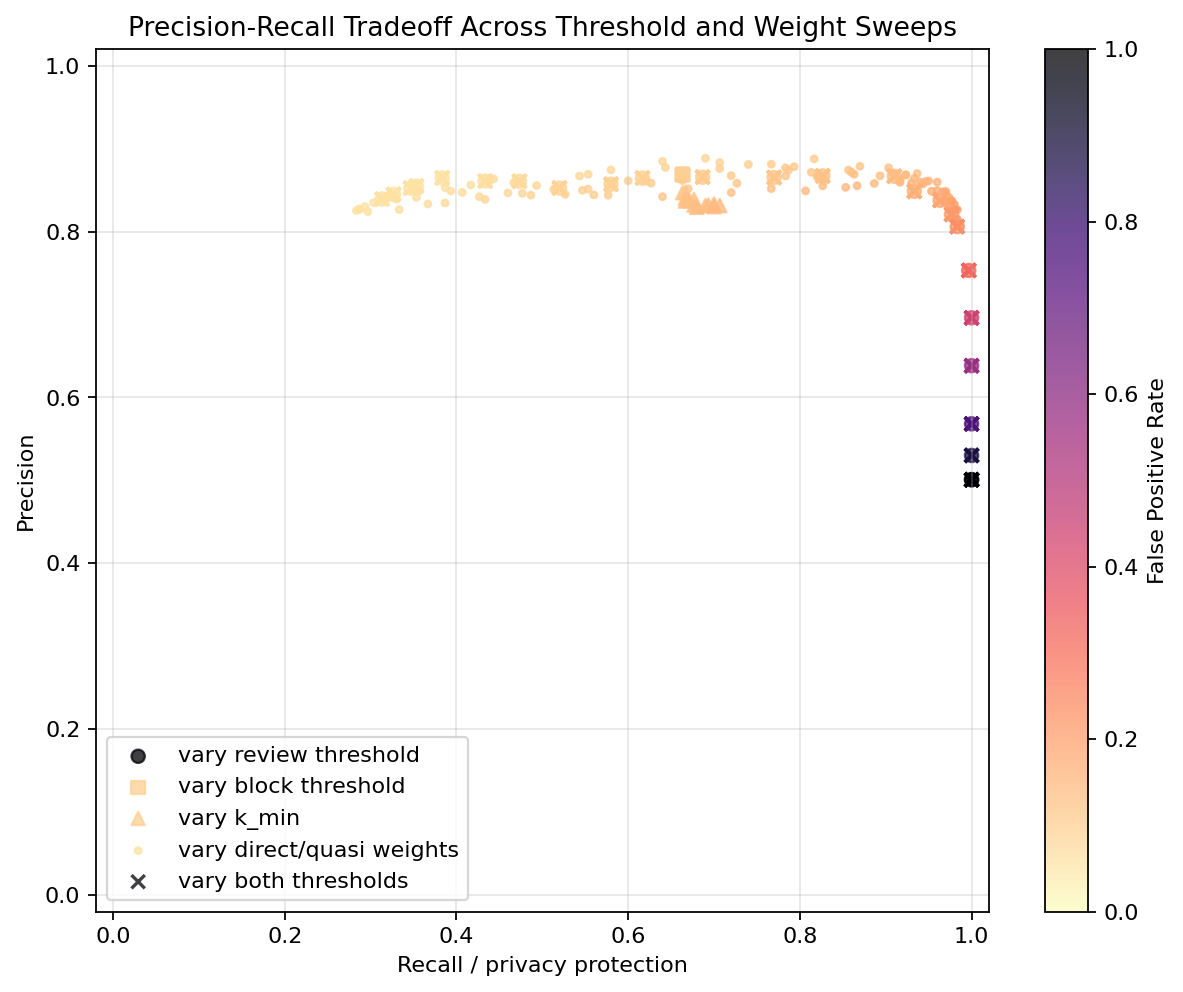
\includegraphics[width=0.9\textwidth]{02_precision_recall_curves.png}
\caption{Precision-recall tradeoff across threshold and weight sweeps.}
\label{fig:pr}
\end{figure}

\subsection{Privacy vs. False Positive Tradeoff}

Figure~\ref{fig:tradeoff} directly compares recall against false positive
rate. This is the main plot for selecting a privacy-preserving operating point
that does not over-flag benign text.

\begin{figure}[H]
\centering
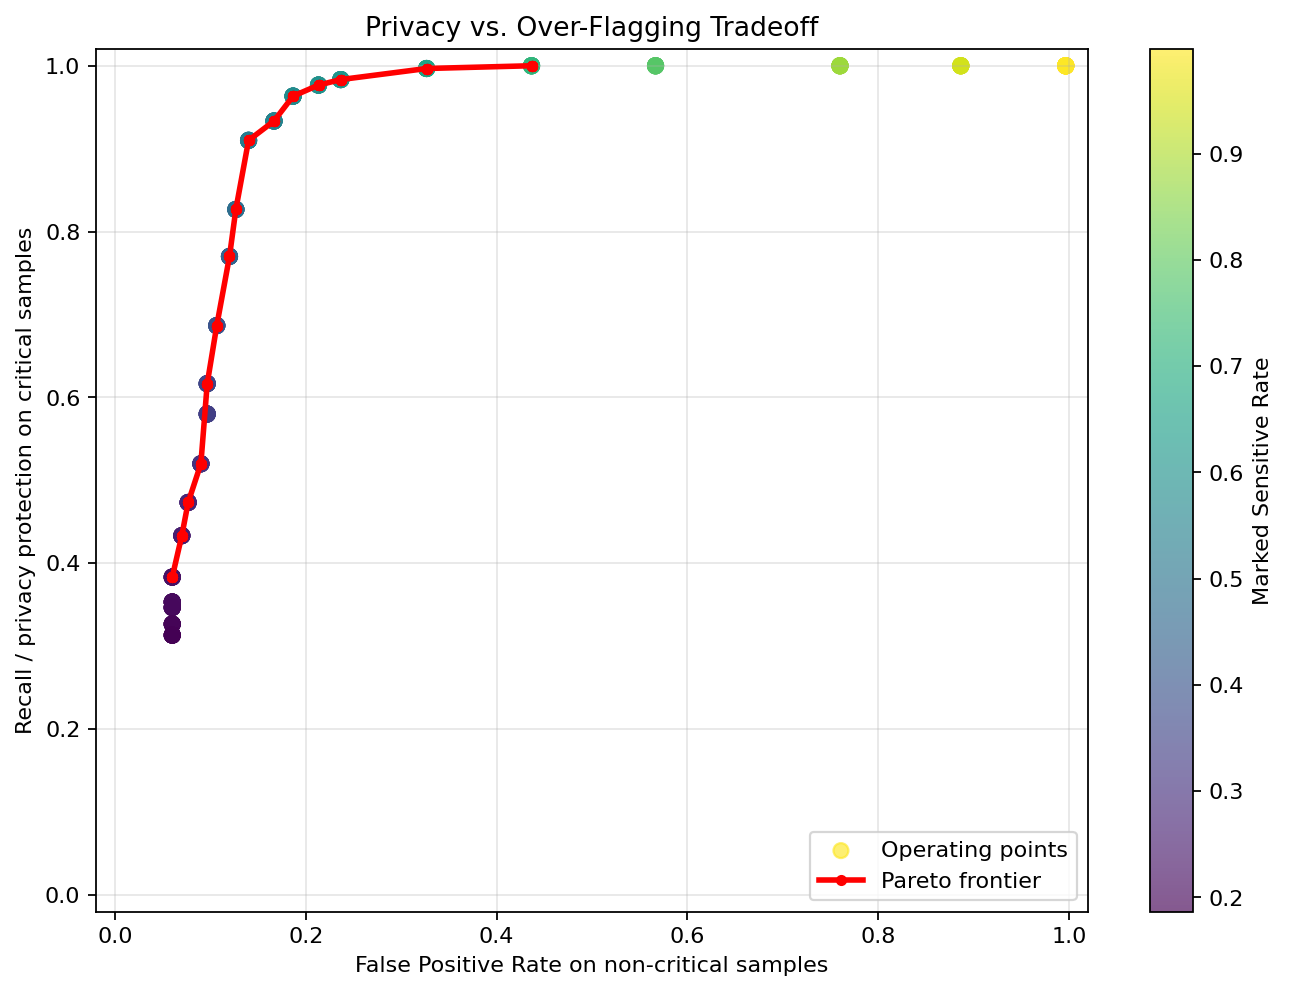
\includegraphics[width=0.9\textwidth]{03_privacy_false_positive_tradeoff.png}
\caption{Privacy recall versus false positive rate.}
\label{fig:tradeoff}
\end{figure}

\subsection{$k_{min}$ Sensitivity}

Figure~\ref{fig:kmin} isolates the effect of the $k_{min}$ threshold. As
$k_{min}$ increases, more samples fail the anonymity floor and are routed to
block. This usually improves privacy protection but can increase false positives.

\begin{figure}[H]
\centering
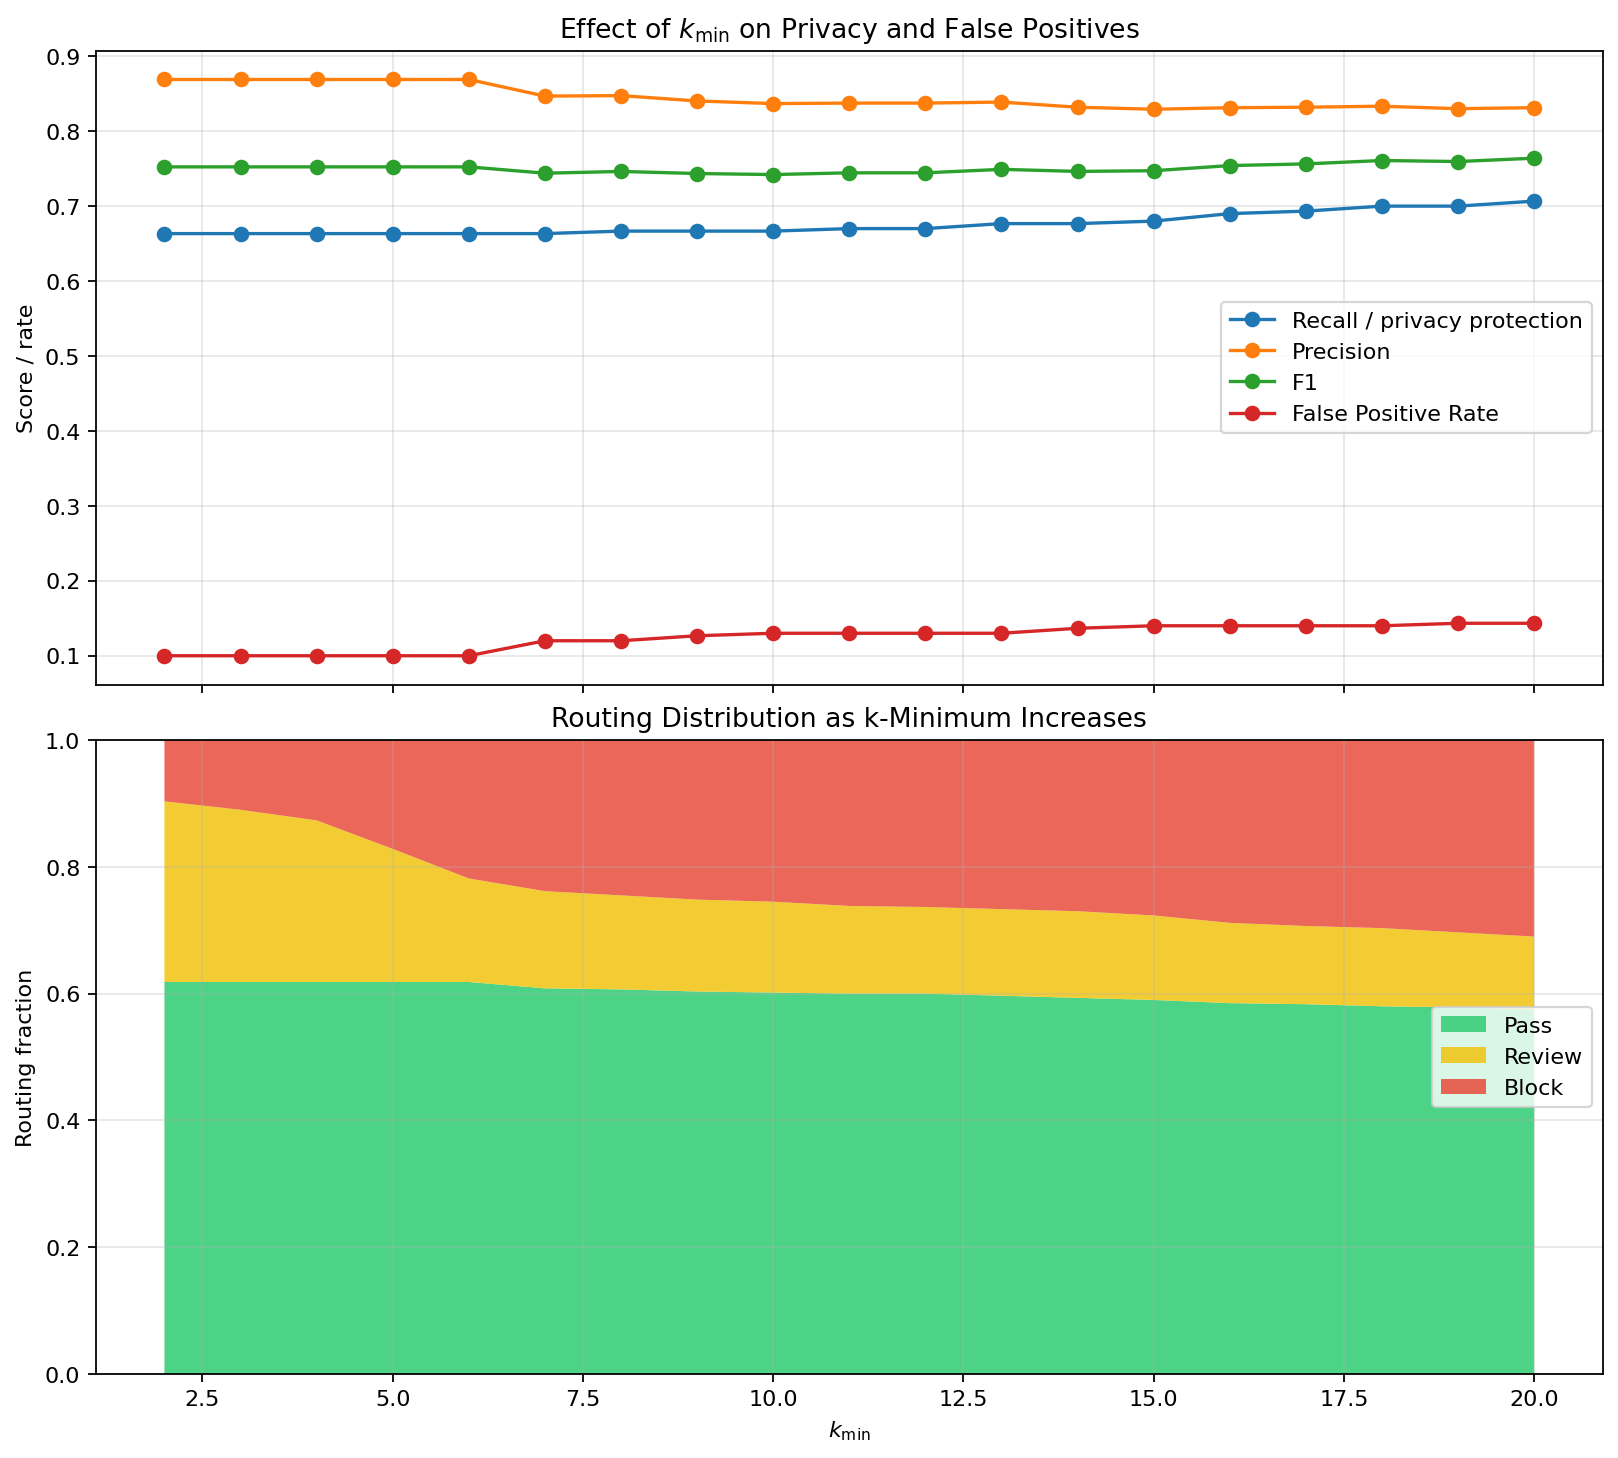
\includegraphics[width=0.9\textwidth]{04_k_minimum_sensitivity.png}
\caption{Sensitivity to the minimum allowable $k$-anonymity lower bound.}
\label{fig:kmin}
\end{figure}

\subsection{Direct and Quasi-Identifier Weights}

Figure~\ref{fig:weights} shows how the direct-identifier and quasi-identifier
weights affect recall, false positive rate, precision, and marked-sensitive
rate. If benign samples contain many entities, high weights may increase
over-flagging.

\begin{figure}[H]
\centering
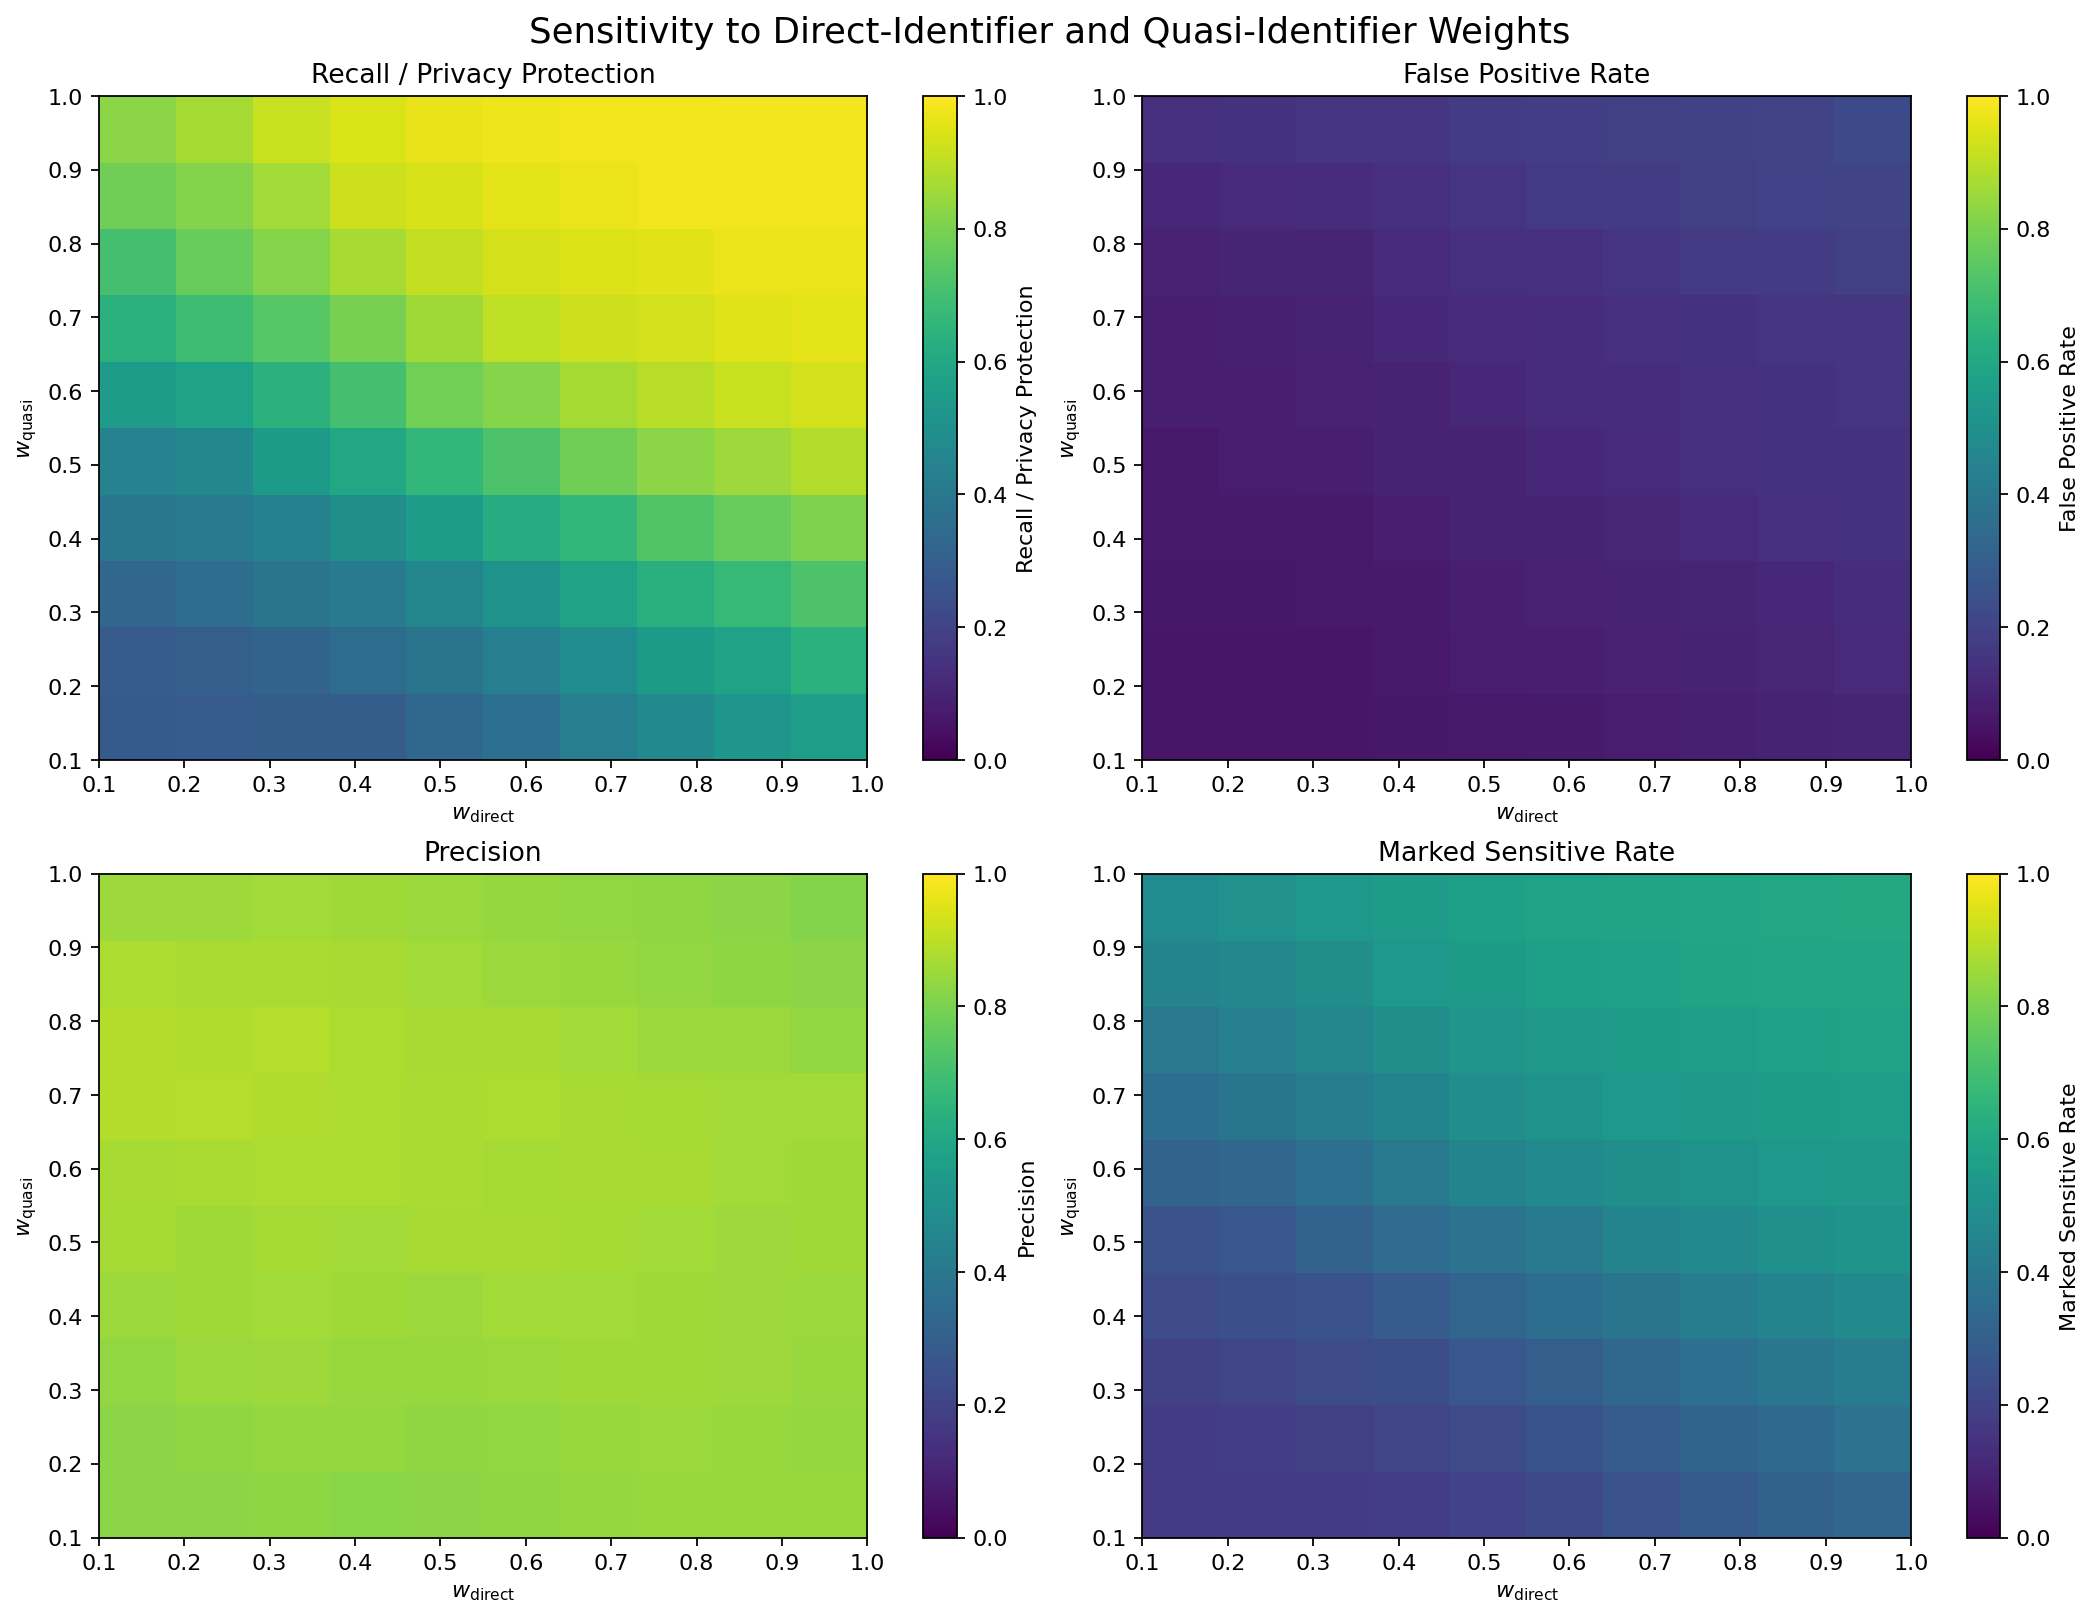
\includegraphics[width=\textwidth]{05_weight_sensitivity_heatmaps.png}
\caption{Sensitivity to direct and quasi-identifier weights.}
\label{fig:weights}
\end{figure}

\subsection{Selected Operating Points}

Figure~\ref{fig:selected} compares selected operating points such as best F1,
best balanced accuracy, high-recall low-FPR, and lowest Wikipedia false positive
rate.

\begin{figure}[H]
\centering
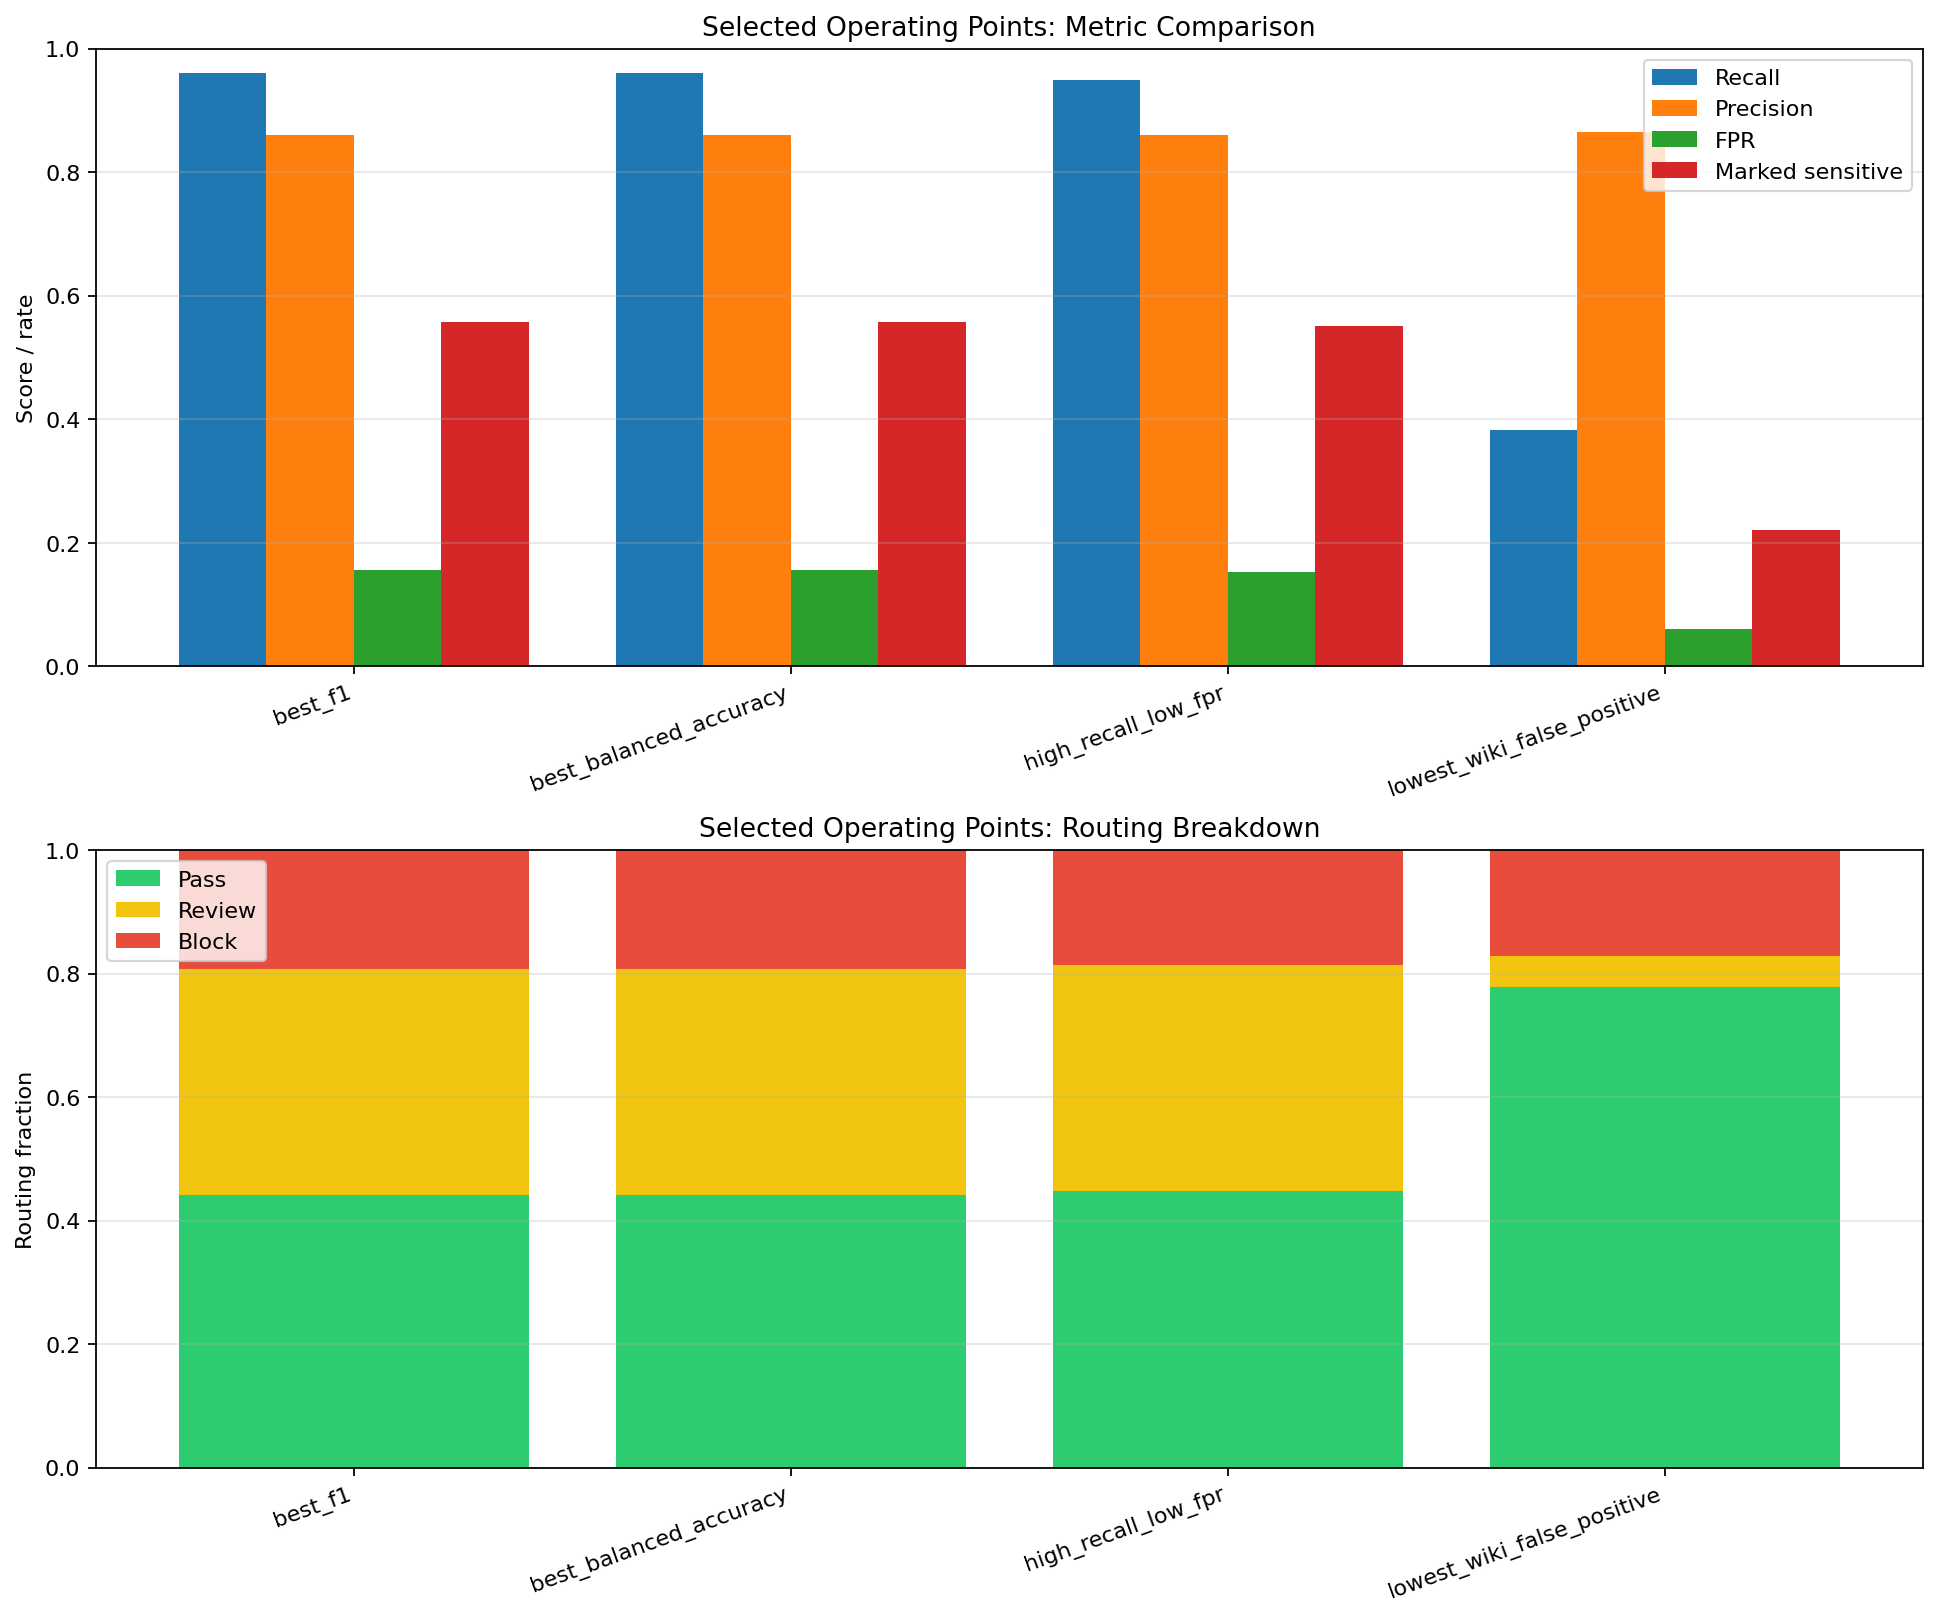
\includegraphics[width=0.95\textwidth]{06_operating_point_breakdown.png}
\caption{Metric and routing breakdown for selected operating points.}
\label{fig:selected}
\end{figure}

\subsection{Wikipedia False Positive Analysis}

Figure~\ref{fig:wiki} focuses on the observed Wikipedia over-flagging problem.
The y-axis is the fraction of Wikipedia samples marked sensitive. The x-axis is
overall privacy recall. The desirable region is low on the y-axis and high on
the x-axis.

\begin{figure}[H]
\centering
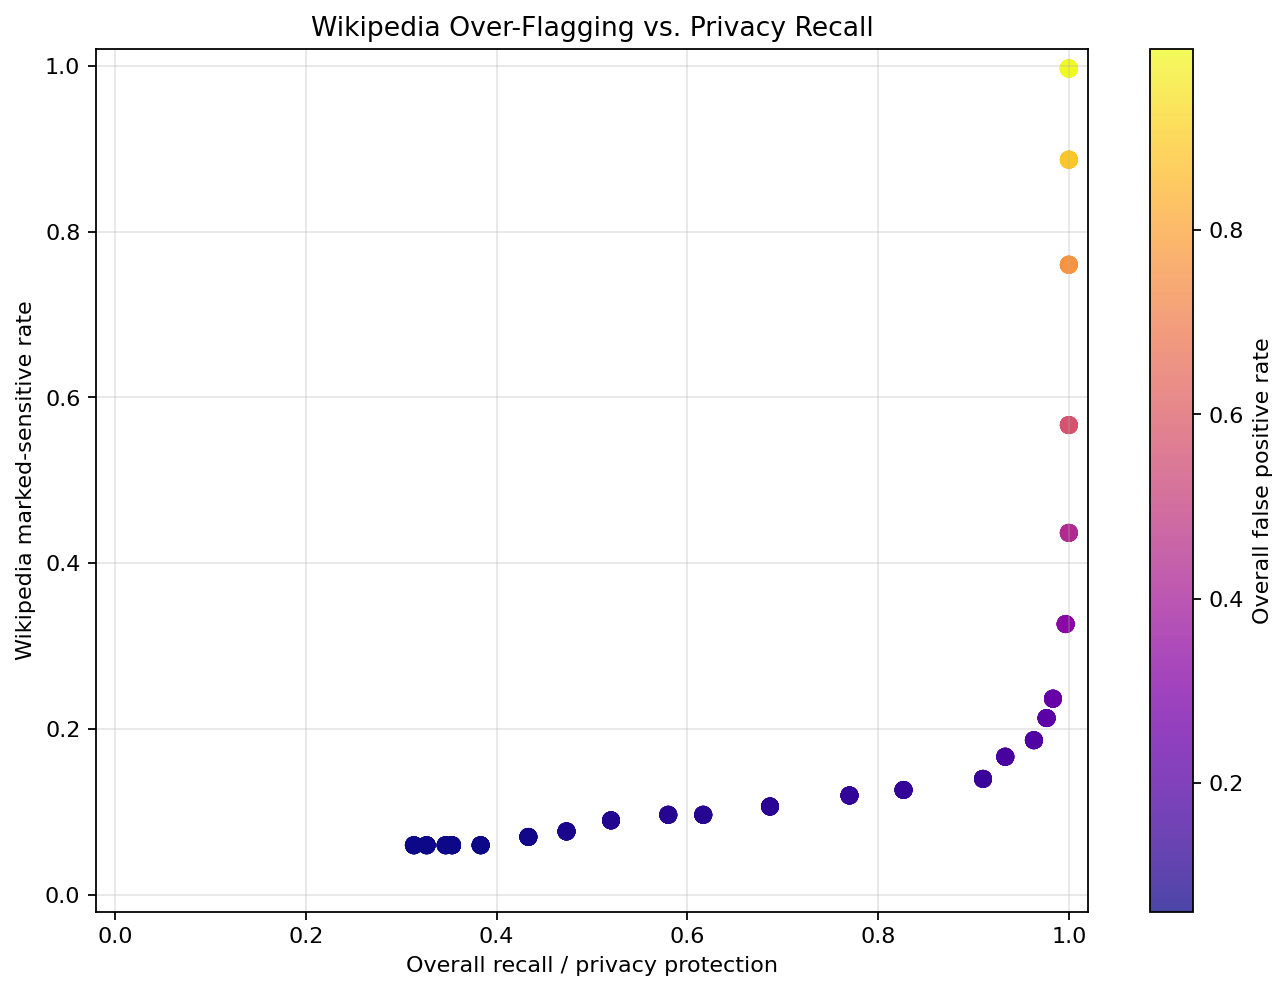
\includegraphics[width=0.9\textwidth]{07_wikipedia_false_positive_analysis.png}
\caption{Wikipedia marked-sensitive rate versus overall privacy recall.}
\label{fig:wiki}
\end{figure}

\section{Selected Operating Points}


\paragraph{Best F1}
This operating point uses
$\tau_{review}=0.30$,
$\tau_{block}=0.70$,
$k_{min}=5$,
$w_{direct}=1.00$, and
$w_{quasi}=0.70$.
It obtains precision $0.860$, recall $0.960$,
F1 $0.907$, false positive rate $0.157$,
and marked-sensitive rate $0.558$.
The routing fractions are pass $0.442$,
review $0.365$, and block $0.193$.



\paragraph{Best Balanced Accuracy}
This operating point uses
$\tau_{review}=0.30$,
$\tau_{block}=0.70$,
$k_{min}=5$,
$w_{direct}=1.00$, and
$w_{quasi}=0.70$.
It obtains precision $0.860$, recall $0.960$,
F1 $0.907$, false positive rate $0.157$,
and marked-sensitive rate $0.558$.
The routing fractions are pass $0.442$,
review $0.365$, and block $0.193$.



\paragraph{High Recall with Low False Positive Rate}
This operating point uses
$\tau_{review}=0.30$,
$\tau_{block}=0.70$,
$k_{min}=5$,
$w_{direct}=0.90$, and
$w_{quasi}=0.70$.
It obtains precision $0.861$, recall $0.950$,
F1 $0.903$, false positive rate $0.153$,
and marked-sensitive rate $0.552$.
The routing fractions are pass $0.448$,
review $0.365$, and block $0.187$.



\paragraph{Lowest Wikipedia False Positive Rate}
This operating point uses
$\tau_{review}=0.41$,
$\tau_{block}=0.70$,
$k_{min}=5$,
$w_{direct}=0.50$, and
$w_{quasi}=0.50$.
It obtains precision $0.865$, recall $0.383$,
F1 $0.531$, false positive rate $0.060$,
and marked-sensitive rate $0.222$.
The routing fractions are pass $0.778$,
review $0.050$, and block $0.172$.


\section{Interpretation}

The analysis separates two competing goals. The first goal is privacy protection:
critical samples should be routed to review or block. This is measured by recall.
The second goal is utility: non-critical samples should not be unnecessarily
marked sensitive. This is measured by false positive rate and by the
Wikipedia-specific marked-sensitive rate.

Lowering $\tau_{review}$ usually increases recall because more samples enter
local review. However, it can also increase false positives. Raising
$\tau_{review}$ usually reduces over-flagging but may miss critical samples.

Lowering $\tau_{block}$ usually increases the block rate. This can strengthen
privacy but may route too many benign samples to the most restrictive path.

Increasing $k_{min}$ makes the anonymity floor stricter. This can prevent
low-anonymity quasi-identifier combinations from passing, but it can also cause
benign entity-rich documents to be treated as sensitive.

Increasing $w_{direct}$ and $w_{quasi}$ increases the influence of detected
identifier counts on the adjusted risk score. If false positives are caused by
entity-rich but non-sensitive text, then reducing these weights may reduce
over-flagging.

\section{Recommended Use}

For selecting an operating point, the most relevant figures are the privacy vs.
false positive tradeoff plot and the Wikipedia false positive analysis. A good
operating point should have high recall, low false positive rate, and low
Wikipedia marked-sensitive rate.

\end{document}
